\documentclass[12pt,a4paper]{article}
\usepackage[utf8]{inputenc}
\usepackage[margin=1in]{geometry}
\usepackage{graphicx}
\usepackage{fancyhdr}
\usepackage{listings}
\usepackage{xcolor}
\usepackage{amsmath}
\usepackage{amsfonts}
\usepackage{amssymb}
\usepackage{hyperref}
\usepackage{float}
\usepackage{tocloft}

% Header and footer
\pagestyle{fancy}
\fancyhf{}
\fancyhead[L]{Lab 5: 3D Transformations and Orthographic Projection}
\fancyhead[R]{\thepage}
\fancyfoot[C]{Computer Graphics Laboratory}

% Code listing style
\definecolor{codegreen}{rgb}{0,0.6,0}
\definecolor{codegray}{rgb}{0.5,0.5,0.5}
\definecolor{codepurple}{rgb}{0.58,0,0.82}
\definecolor{backcolour}{rgb}{0.95,0.95,0.92}

\lstdefinestyle{mystyle}{
    backgroundcolor=\color{backcolour},   
    commentstyle=\color{codegreen},
    keywordstyle=\color{magenta},
    numberstyle=\tiny\color{codegray},
    stringstyle=\color{codepurple},
    basicstyle=\ttfamily\footnotesize,
    breakatwhitespace=false,         
    breaklines=true,                 
    captionpos=b,                    
    keepspaces=true,                 
    numbers=left,                    
    numbersep=5pt,                  
    showspaces=false,                
    showstringspaces=false,
    showtabs=false,                  
    tabsize=2
}

\lstset{style=mystyle}

\begin{document}

% Title Page
\begin{titlepage}
    \centering
    \vspace*{0.5cm}
    
    \Huge
    \textbf{Computer Graphics Laboratory}
    
    \vspace{0.5cm}
    \LARGE
    Lab Report 5
    
    \vspace{1.5cm}
    
    \textbf{\huge 3D Transformations and Orthographic Projection}
    
    \vspace{4cm}
    % \includegraphics[width=0.4\textwidth]{logo.png}
    
    \vspace{2cm}
    
    \Large
    \textbf{Student Name:} [Your Name]\\
    \textbf{Roll Number:} [Your Roll Number]\\
    \textbf{Course:} Computer Graphics\\
    \textbf{Semester:} 5th\\
    
    \vfill
    
    \large
    Department of Computer Science and Engineering\\
    [Your University Name]\\
    \today
    
\end{titlepage}

% Table of Contents
\tableofcontents
\newpage

\section{Title of Lab Activity}

\subsection{Objective}
To implement 3D transformations including Translation, Rotation, Scaling, and Shearing using OpenGL, and to demonstrate the difference between Orthographic and Perspective projections for 3D object rendering.

\subsection{Problem Statement}
Write programs to implement the following 3D transformations using OpenGL:
\begin{itemize}
    \item 3D Translation
    \item 3D Rotation (about X, Y, Z axes)
    \item 3D Scaling
    \item 3D Shearing (all six components: xy, xz, yx, yz, zx, zy)
    \item Orthographic vs Perspective Projection visualization
\end{itemize}

The implementation should provide interactive controls to apply these transformations to standard 3D shapes (cube, sphere, teapot, torus) and allow real-time switching between projection modes.

\section{Algorithm Used for 3D Transformations and Projections}

\subsection{3D Translation}
Translation moves a point or object from one location to another in 3D space. The transformation is defined by displacement values along the X, Y, and Z axes.

\textbf{Mathematical Formulation:}
\begin{align}
\begin{bmatrix}
x' \\
y' \\
z' \\
1
\end{bmatrix}
=
\begin{bmatrix}
1 & 0 & 0 & t_x \\
0 & 1 & 0 & t_y \\
0 & 0 & 1 & t_z \\
0 & 0 & 0 & 1
\end{bmatrix}
\begin{bmatrix}
x \\
y \\
z \\
1
\end{bmatrix}
\end{align}

Where $(t_x, t_y, t_z)$ are the translation distances along the respective axes.

\subsection{3D Rotation}
3D rotation rotates an object about the X, Y, or Z axes by specified angles.

\textbf{Rotation about X-axis:}
\begin{align}
R_x(\theta) = \begin{bmatrix}
1 & 0 & 0 & 0 \\
0 & \cos\theta & -\sin\theta & 0 \\
0 & \sin\theta & \cos\theta & 0 \\
0 & 0 & 0 & 1
\end{bmatrix}
\end{align}

\textbf{Rotation about Y-axis:}
\begin{align}
R_y(\theta) = \begin{bmatrix}
\cos\theta & 0 & \sin\theta & 0 \\
0 & 1 & 0 & 0 \\
-\sin\theta & 0 & \cos\theta & 0 \\
0 & 0 & 0 & 1
\end{bmatrix}
\end{align}

\textbf{Rotation about Z-axis:}
\begin{align}
R_z(\theta) = \begin{bmatrix}
\cos\theta & -\sin\theta & 0 & 0 \\
\sin\theta & \cos\theta & 0 & 0 \\
0 & 0 & 1 & 0 \\
0 & 0 & 0 & 1
\end{bmatrix}
\end{align}

\subsection{3D Scaling}
Scaling changes the size of an object along the X, Y, and Z axes.

\textbf{Mathematical Formulation:}
\begin{align}
S(s_x, s_y, s_z) = \begin{bmatrix}
s_x & 0 & 0 & 0 \\
0 & s_y & 0 & 0 \\
0 & 0 & s_z & 0 \\
0 & 0 & 0 & 1
\end{bmatrix}
\end{align}

Where $(s_x, s_y, s_z)$ are the scaling factors along the respective axes.

\subsection{3D Shearing}
3D shearing transformation skews the shape of an object. The general 3D shearing matrix includes six shearing parameters.

\textbf{Mathematical Formulation:}
\begin{align}
H = \begin{bmatrix}
1 & h_{yx} & h_{zx} & 0 \\
h_{xy} & 1 & h_{zy} & 0 \\
h_{xz} & h_{yz} & 1 & 0 \\
0 & 0 & 0 & 1
\end{bmatrix}
\end{align}

Where $h_{ij}$ represents the shearing of coordinate $i$ with respect to coordinate $j$.

\subsection{Interactive Controls Algorithm}

\textbf{OpenGL Transformation Pipeline:}
\begin{enumerate}
    \item Initialize OpenGL context with depth testing and lighting
    \item Set up projection matrix (perspective or orthographic)
    \item Apply modelview transformations in sequence:
    \begin{itemize}
        \item Translation: \texttt{glTranslatef(tx, ty, tz)}
        \item Shearing: \texttt{glMultMatrixf(shear\_matrix)}
        \item Rotation: \texttt{glRotatef(angle, axis\_x, axis\_y, axis\_z)}
        \item Scaling: \texttt{glScalef(sx, sy, sz)}
    \end{itemize}
    \item Render 3D object using GLUT primitives
    \item Handle user input for real-time manipulation
\end{enumerate}

\subsection{Orthographic vs Perspective Projection}

\textbf{Orthographic Projection:}
Parallel projection where the projection rays are parallel to each other and perpendicular to the projection plane. Object size remains constant regardless of distance from the viewer.

\begin{align}
\text{glOrtho}(left, right, bottom, top, near, far)
\end{align}

\textbf{Perspective Projection:}
Projection that mimics human vision where objects appear smaller as they get farther from the viewer.

\begin{align}
\text{gluPerspective}(fovy, aspect, near, far)
\end{align}

\section{Source Code}

\subsection{Main Implementation (main.py)}
\begin{lstlisting}[language=Python, caption=Complete 3D Transformations with Interactive Controls]
from OpenGL.GL import *
from OpenGL.GLU import *
from OpenGL.GLUT import *

window_width = 1000
window_height = 700

mode = "translate"
axis = "x"
shape_index = 0

tx, ty, tz = 0.0, 0.0, 0.0
rx, ry, rz = 0.0, 0.0, 0.0
sx, sy, sz = 1.0, 1.0, 1.0

shear_components = ["xy", "xz", "yx", "yz", "zx", "zy"]
shear_comp_index = 0
sh_xy = 0.0
sh_xz = 0.0
sh_yx = 0.0
sh_yz = 0.0
sh_zx = 0.0
sh_zy = 0.0

projection = "perspective"

def get_shear_matrix():
    return [
        1.0, sh_yx, sh_zx, 0.0,
        sh_xy, 1.0, sh_zy, 0.0,
        sh_xz, sh_yz, 1.0, 0.0,
        0.0, 0.0, 0.0, 1.0,
    ]

def draw_axes():
    glDisable(GL_LIGHTING)
    glBegin(GL_LINES)
    glColor3f(1, 0, 0)
    glVertex3f(0, 0, 0)
    glVertex3f(2, 0, 0)
    glColor3f(0, 1, 0)
    glVertex3f(0, 0, 0)
    glVertex3f(0, 2, 0)
    glColor3f(0, 0, 1)
    glVertex3f(0, 0, 0)
    glVertex3f(0, 0, 2)
    glEnd()
    glEnable(GL_LIGHTING)

def draw_shape():
    glColor3f(0.9, 0.9, 0.9)
    if shape_index == 0:
        glutSolidCube(1.0)
    elif shape_index == 1:
        glutSolidSphere(0.6, 32, 32)
    elif shape_index == 2:
        glutSolidTeapot(0.6)
    else:
        glutSolidTorus(0.2, 0.6, 32, 32)

def display():
    glClear(GL_COLOR_BUFFER_BIT | GL_DEPTH_BUFFER_BIT)

    glMatrixMode(GL_PROJECTION)
    glLoadIdentity()
    aspect = window_width / float(window_height)
    if projection == "perspective":
        gluPerspective(60.0, aspect, 0.1, 100.0)
    else:
        glOrtho(-2.0 * aspect, 2.0 * aspect, -2.0, 2.0, 0.1, 100.0)

    glMatrixMode(GL_MODELVIEW)
    glLoadIdentity()
    gluLookAt(0.0, 0.0, 4.0, 0.0, 0.0, 0.0, 0.0, 1.0, 0.0)

    draw_axes()

    glPushMatrix()
    # Apply transformations in sequence
    glTranslatef(tx, ty, tz)
    glMultMatrixf(get_shear_matrix())
    glRotatef(rx, 1, 0, 0)
    glRotatef(ry, 0, 1, 0)
    glRotatef(rz, 0, 0, 1)
    glScalef(sx, sy, sz)
    draw_shape()
    glPopMatrix()

    glutSwapBuffers()
\end{lstlisting}

\subsection{3D Rotation Implementation (rotation.py)}
\begin{lstlisting}[language=Python, caption=Dedicated 3D Rotation Implementation]
from OpenGL.GL import *
from OpenGL.GLU import *
from OpenGL.GLUT import *

axis = "x"
shape_index = 0
rx, ry, rz = 0.0, 0.0, 0.0

def display():
    glClear(GL_COLOR_BUFFER_BIT | GL_DEPTH_BUFFER_BIT)

    glMatrixMode(GL_PROJECTION)
    glLoadIdentity()
    aspect = window_width / float(window_height)
    gluPerspective(60.0, aspect, 0.1, 100.0)

    glMatrixMode(GL_MODELVIEW)
    glLoadIdentity()
    gluLookAt(0.0, 0.0, 4.0, 0.0, 0.0, 0.0, 0.0, 1.0, 0.0)

    draw_axes()

    glPushMatrix()
    # Apply rotations about each axis
    glRotatef(rx, 1, 0, 0)  # Rotation about X-axis
    glRotatef(ry, 0, 1, 0)  # Rotation about Y-axis
    glRotatef(rz, 0, 0, 1)  # Rotation about Z-axis
    draw_shape()
    glPopMatrix()

    glutSwapBuffers()
\end{lstlisting}

\subsection{Visual Output Generation}
\begin{lstlisting}[language=Python, caption=Static Visualization Generator (visual\_demo.py)]
def plot_3d_transformation(original_vertices, transformed_vertices, title, filename):
    """Plot original and transformed 3D objects"""
    fig = plt.figure(figsize=(15, 6))
    
    # Original object
    ax1 = fig.add_subplot(121, projection='3d')
    poly3d_orig = Poly3DCollection(faces_orig_updated, alpha=0.7, 
                                   facecolor='lightblue', edgecolor='black')
    ax1.add_collection3d(poly3d_orig)
    
    # Transformed object  
    ax2 = fig.add_subplot(122, projection='3d')
    poly3d_trans = Poly3DCollection(faces_trans_updated, alpha=0.7,
                                    facecolor='lightgreen', edgecolor='black')
    ax2.add_collection3d(poly3d_trans)
    
    plt.suptitle(title, fontsize=14, fontweight='bold')
    plt.savefig(f'fig/{filename}', dpi=300, bbox_inches='tight')

def generate_all_transformations():
    """Generate all transformation visualizations"""
    vertices, _ = create_cube()
    
    # Generate transformation matrices and apply them
    trans_matrix = translation_matrix(1.0, 0.5, 0.8)
    rot_matrix = rotation_matrix_y(np.pi/4) @ rotation_matrix_x(np.pi/6)
    scale_matrix = scaling_matrix(1.5, 0.8, 2.0)
    shear_matrix = shearing_matrix(hxy=0.3, hyz=0.2)
    
    # Plot comparisons for each transformation type
\end{lstlisting}

\section{Output}

\subsection{3D Translation Output}
\begin{figure}[H]
    \centering
    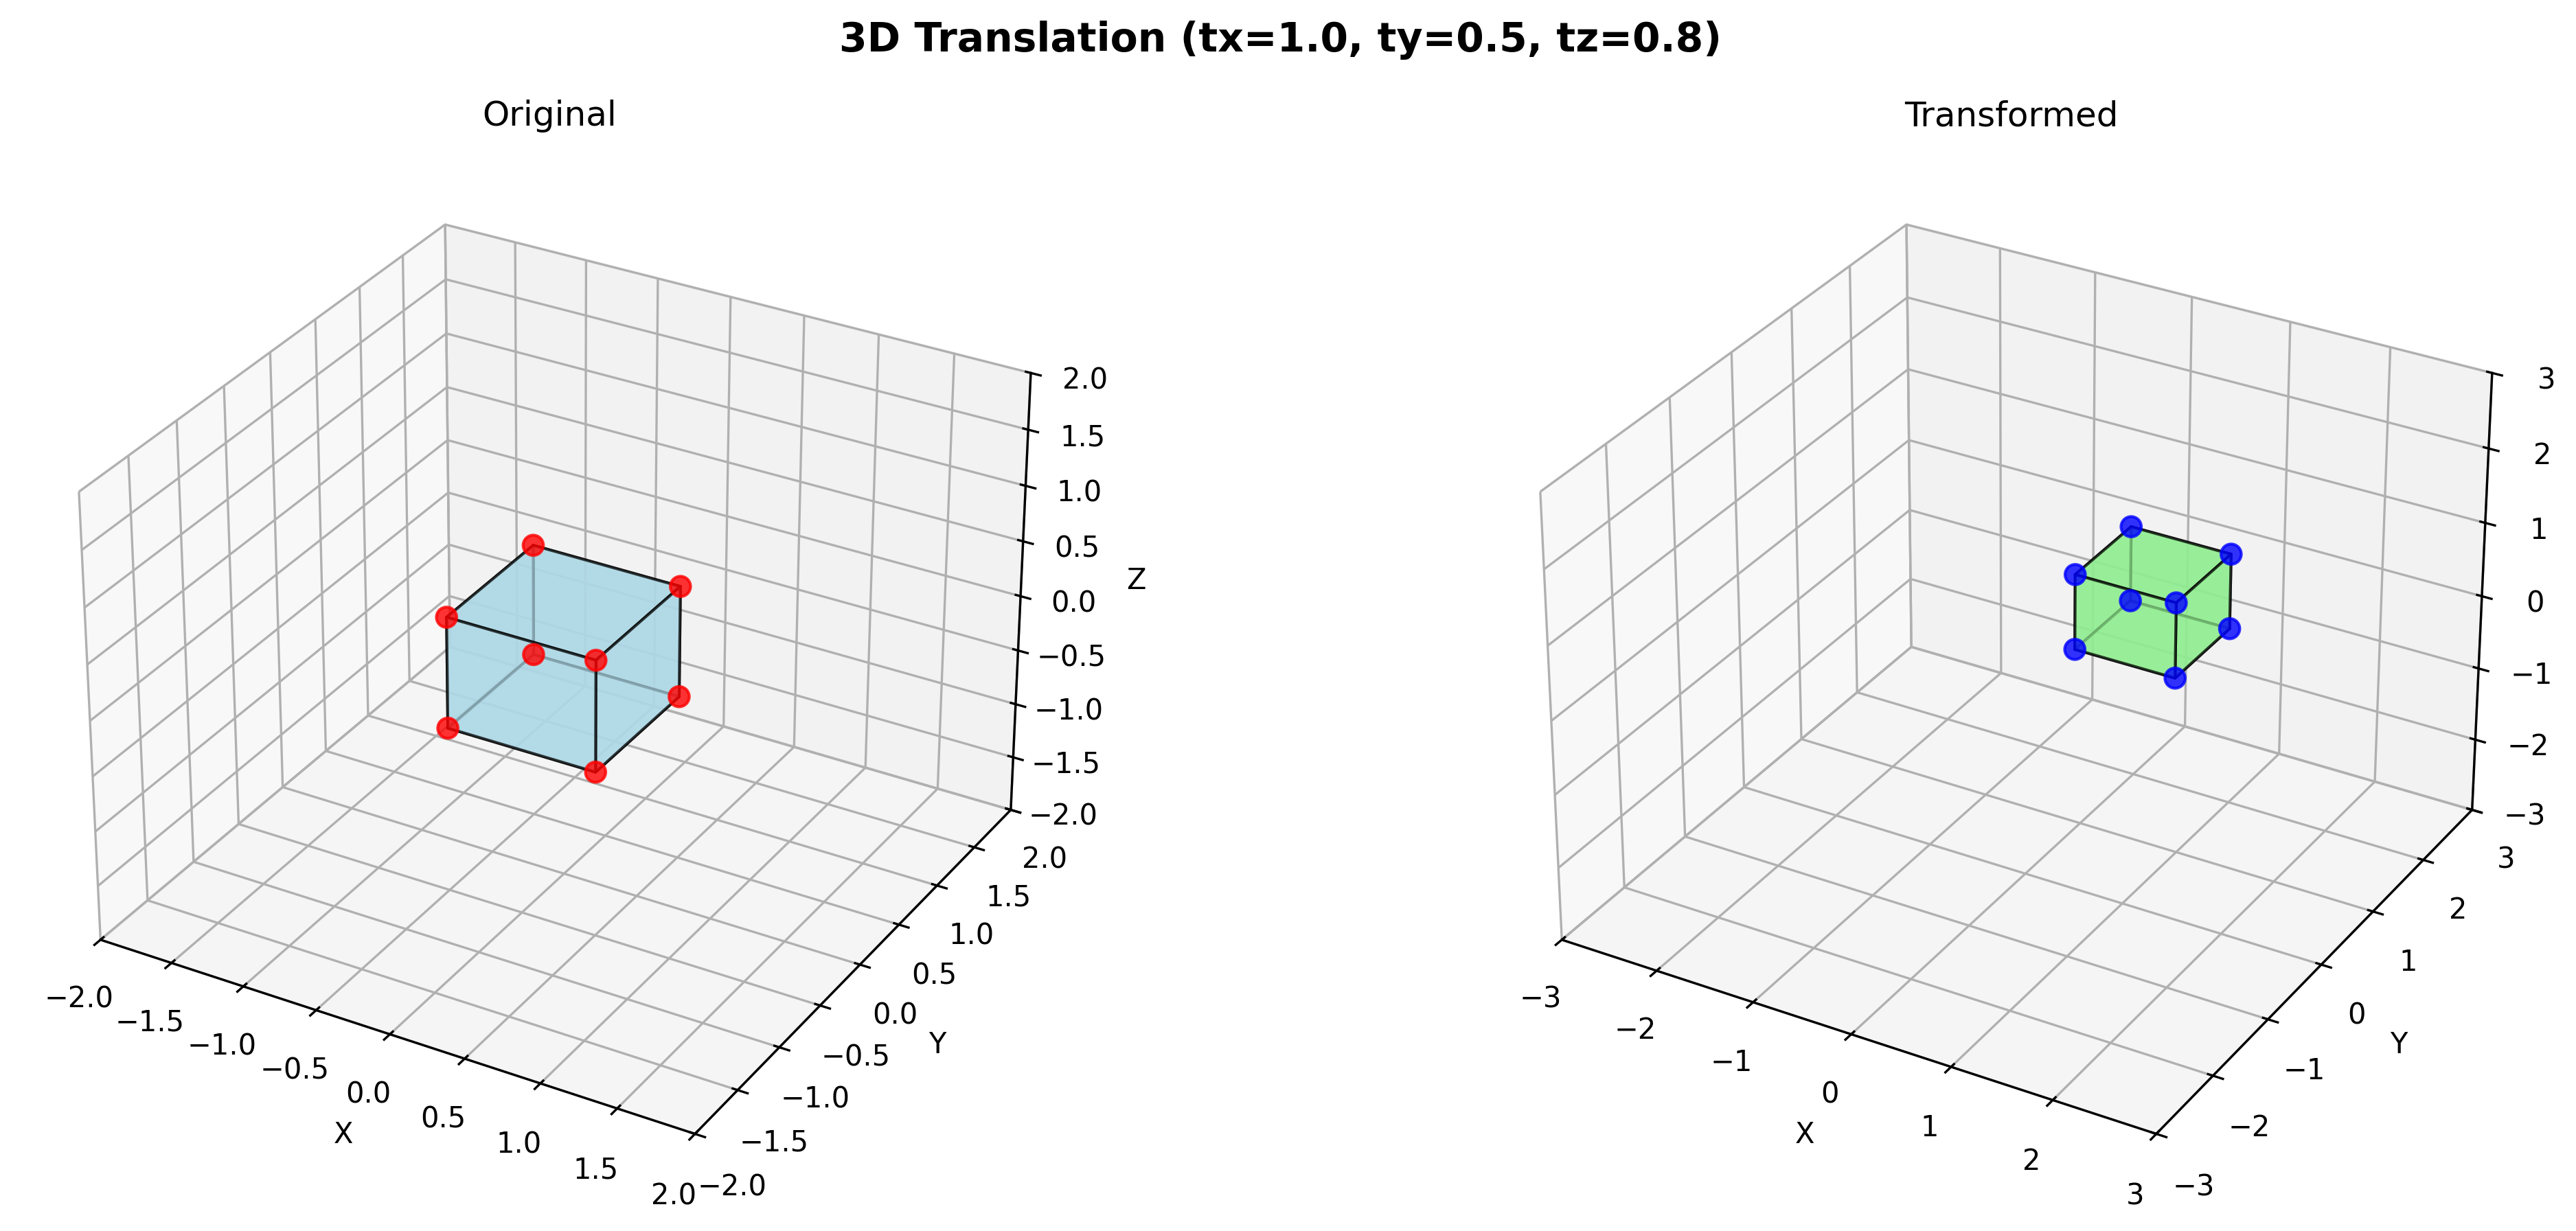
\includegraphics[width=0.8\textwidth]{fig/translation_demo.png}
    \caption{3D Translation demonstration showing object movement along X, Y, and Z axes}
\end{figure}

\subsection{3D Rotation Output}
\begin{figure}[H]
    \centering
    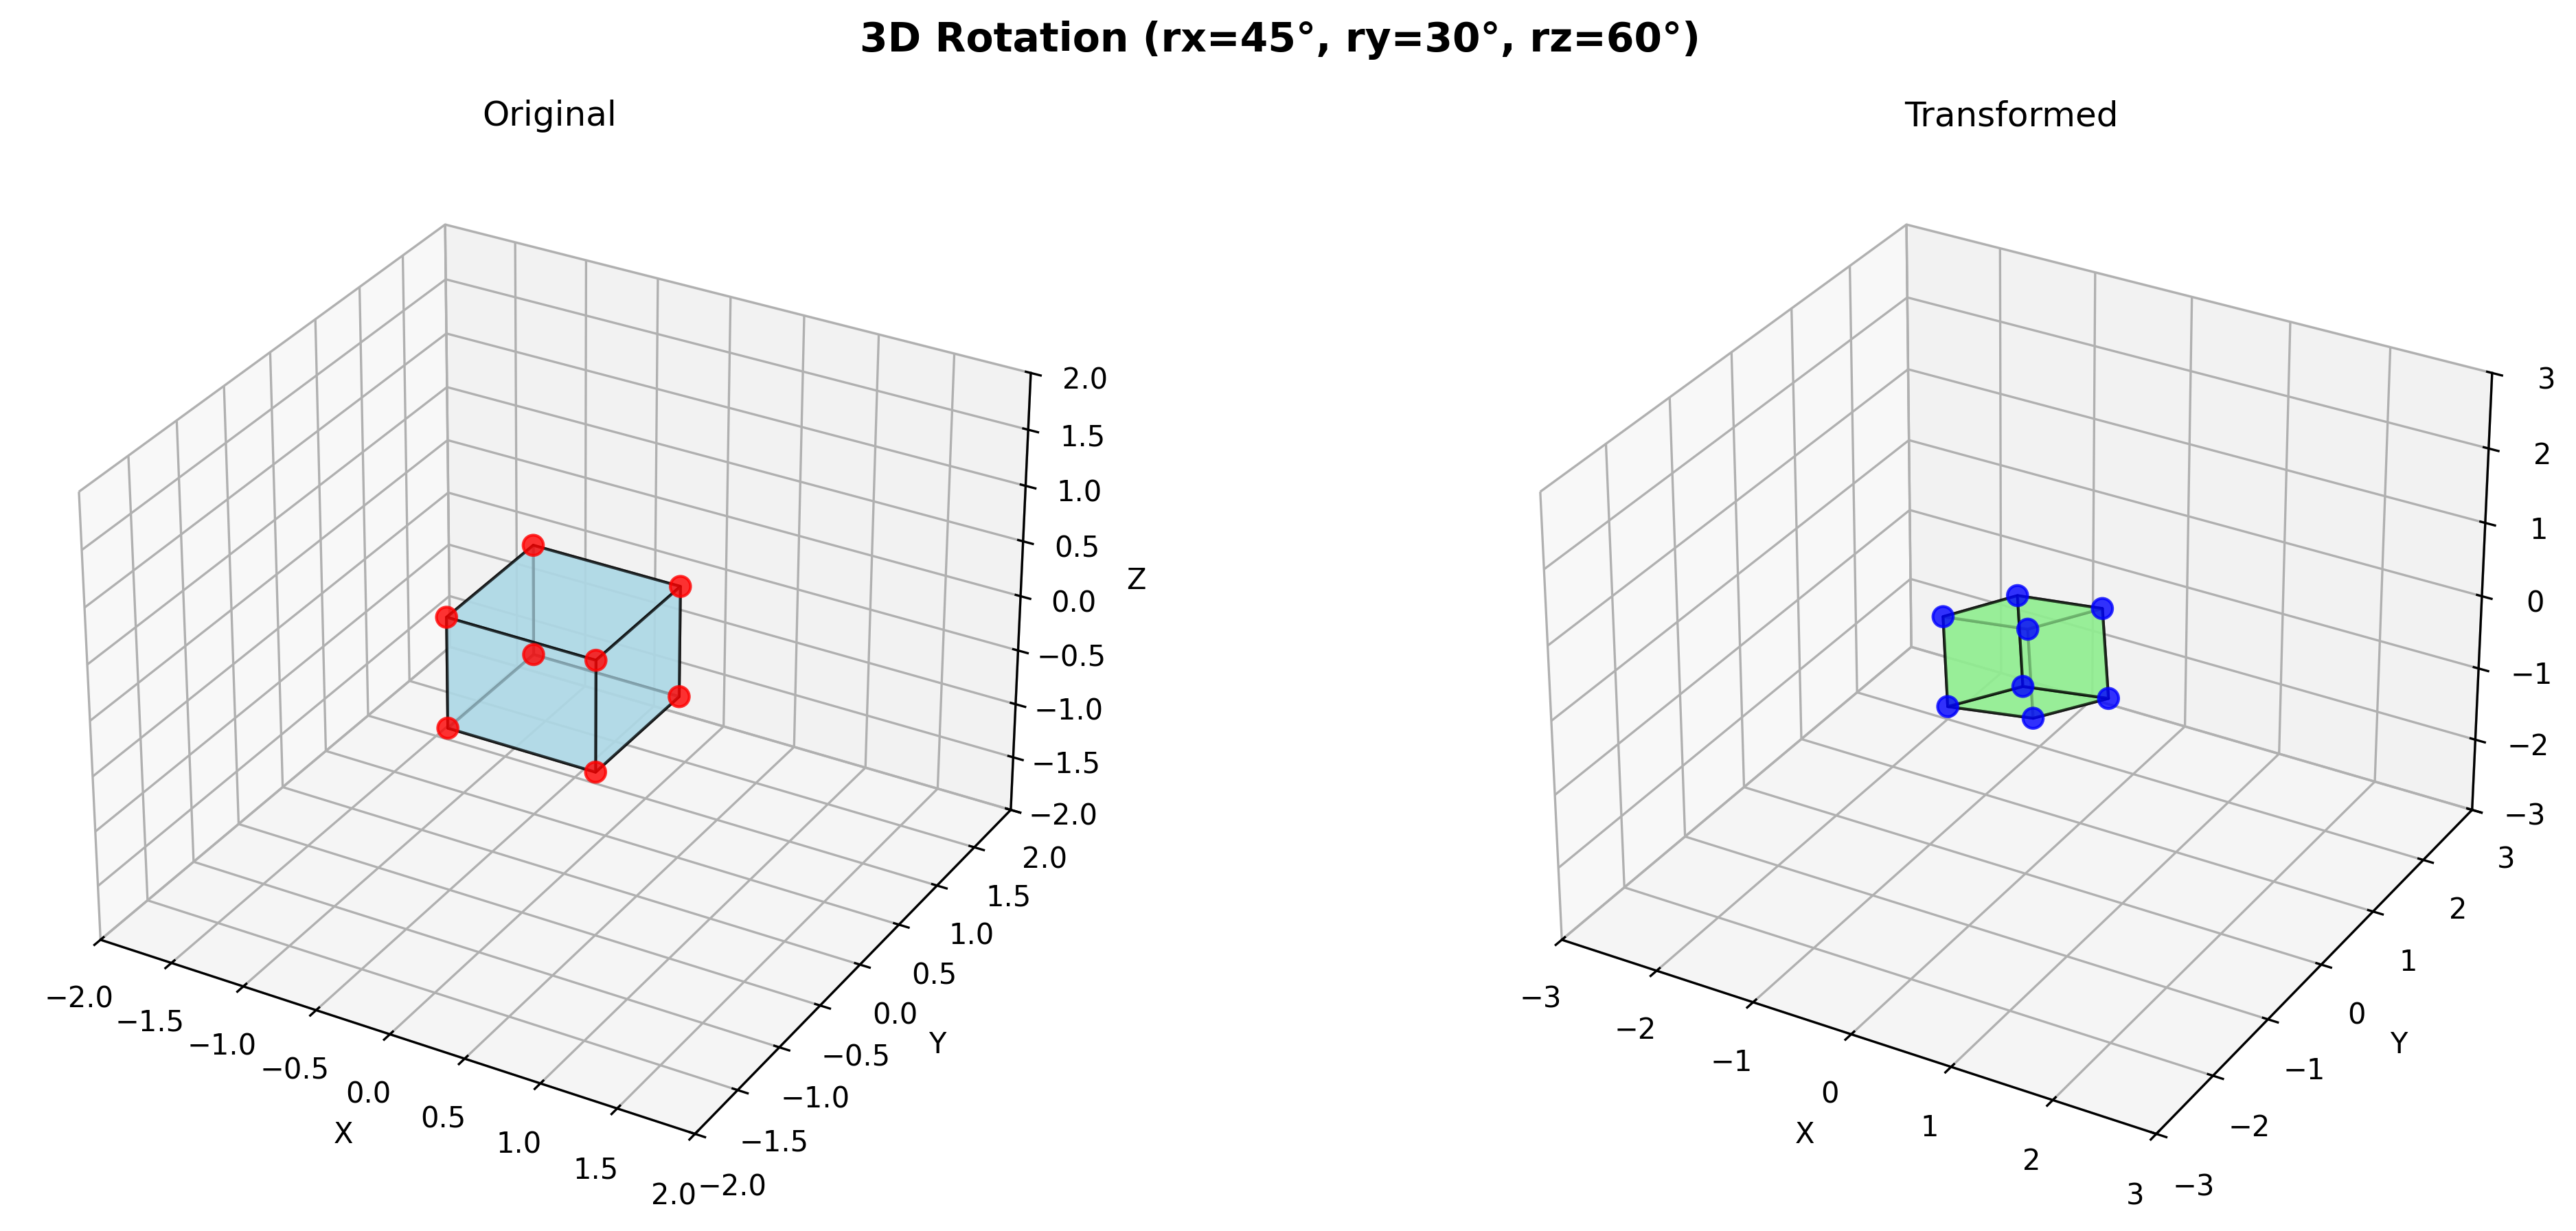
\includegraphics[width=0.8\textwidth]{fig/rotation_demo.png}
    \caption{3D Rotation demonstration showing rotation about X, Y, and Z axes}
\end{figure}

\subsection{3D Scaling Output}
\begin{figure}[H]
    \centering
    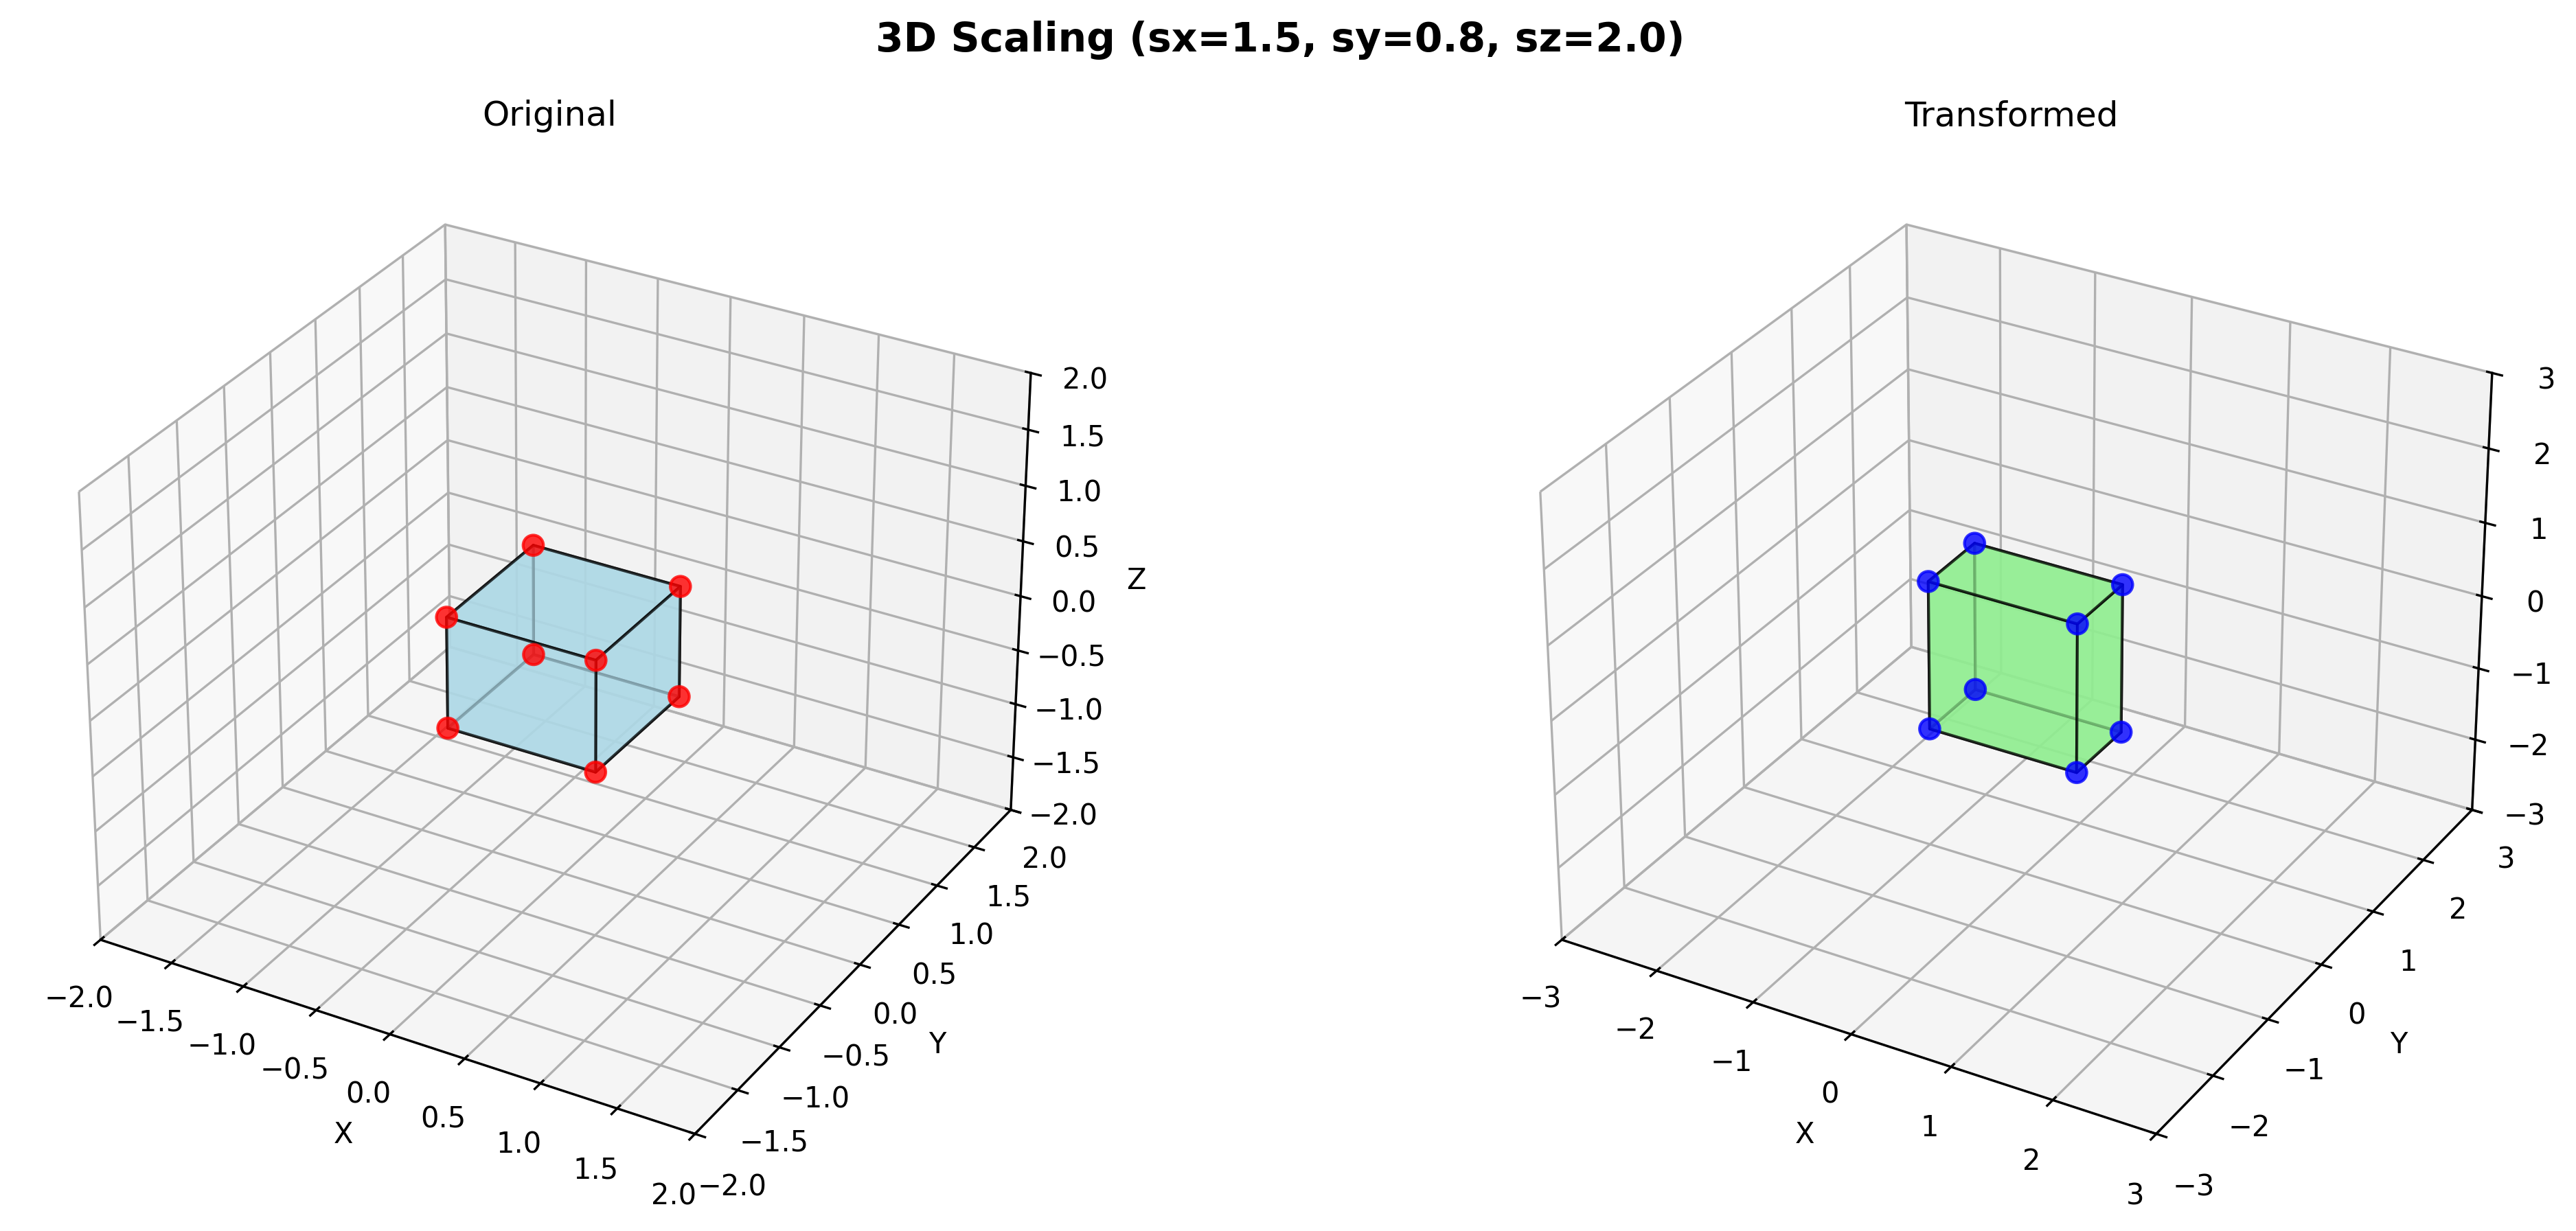
\includegraphics[width=0.8\textwidth]{fig/scaling_demo.png}
    \caption{3D Scaling demonstration showing uniform and non-uniform scaling}
\end{figure}

\subsection{3D Shearing Output}
\begin{figure}[H]
    \centering
    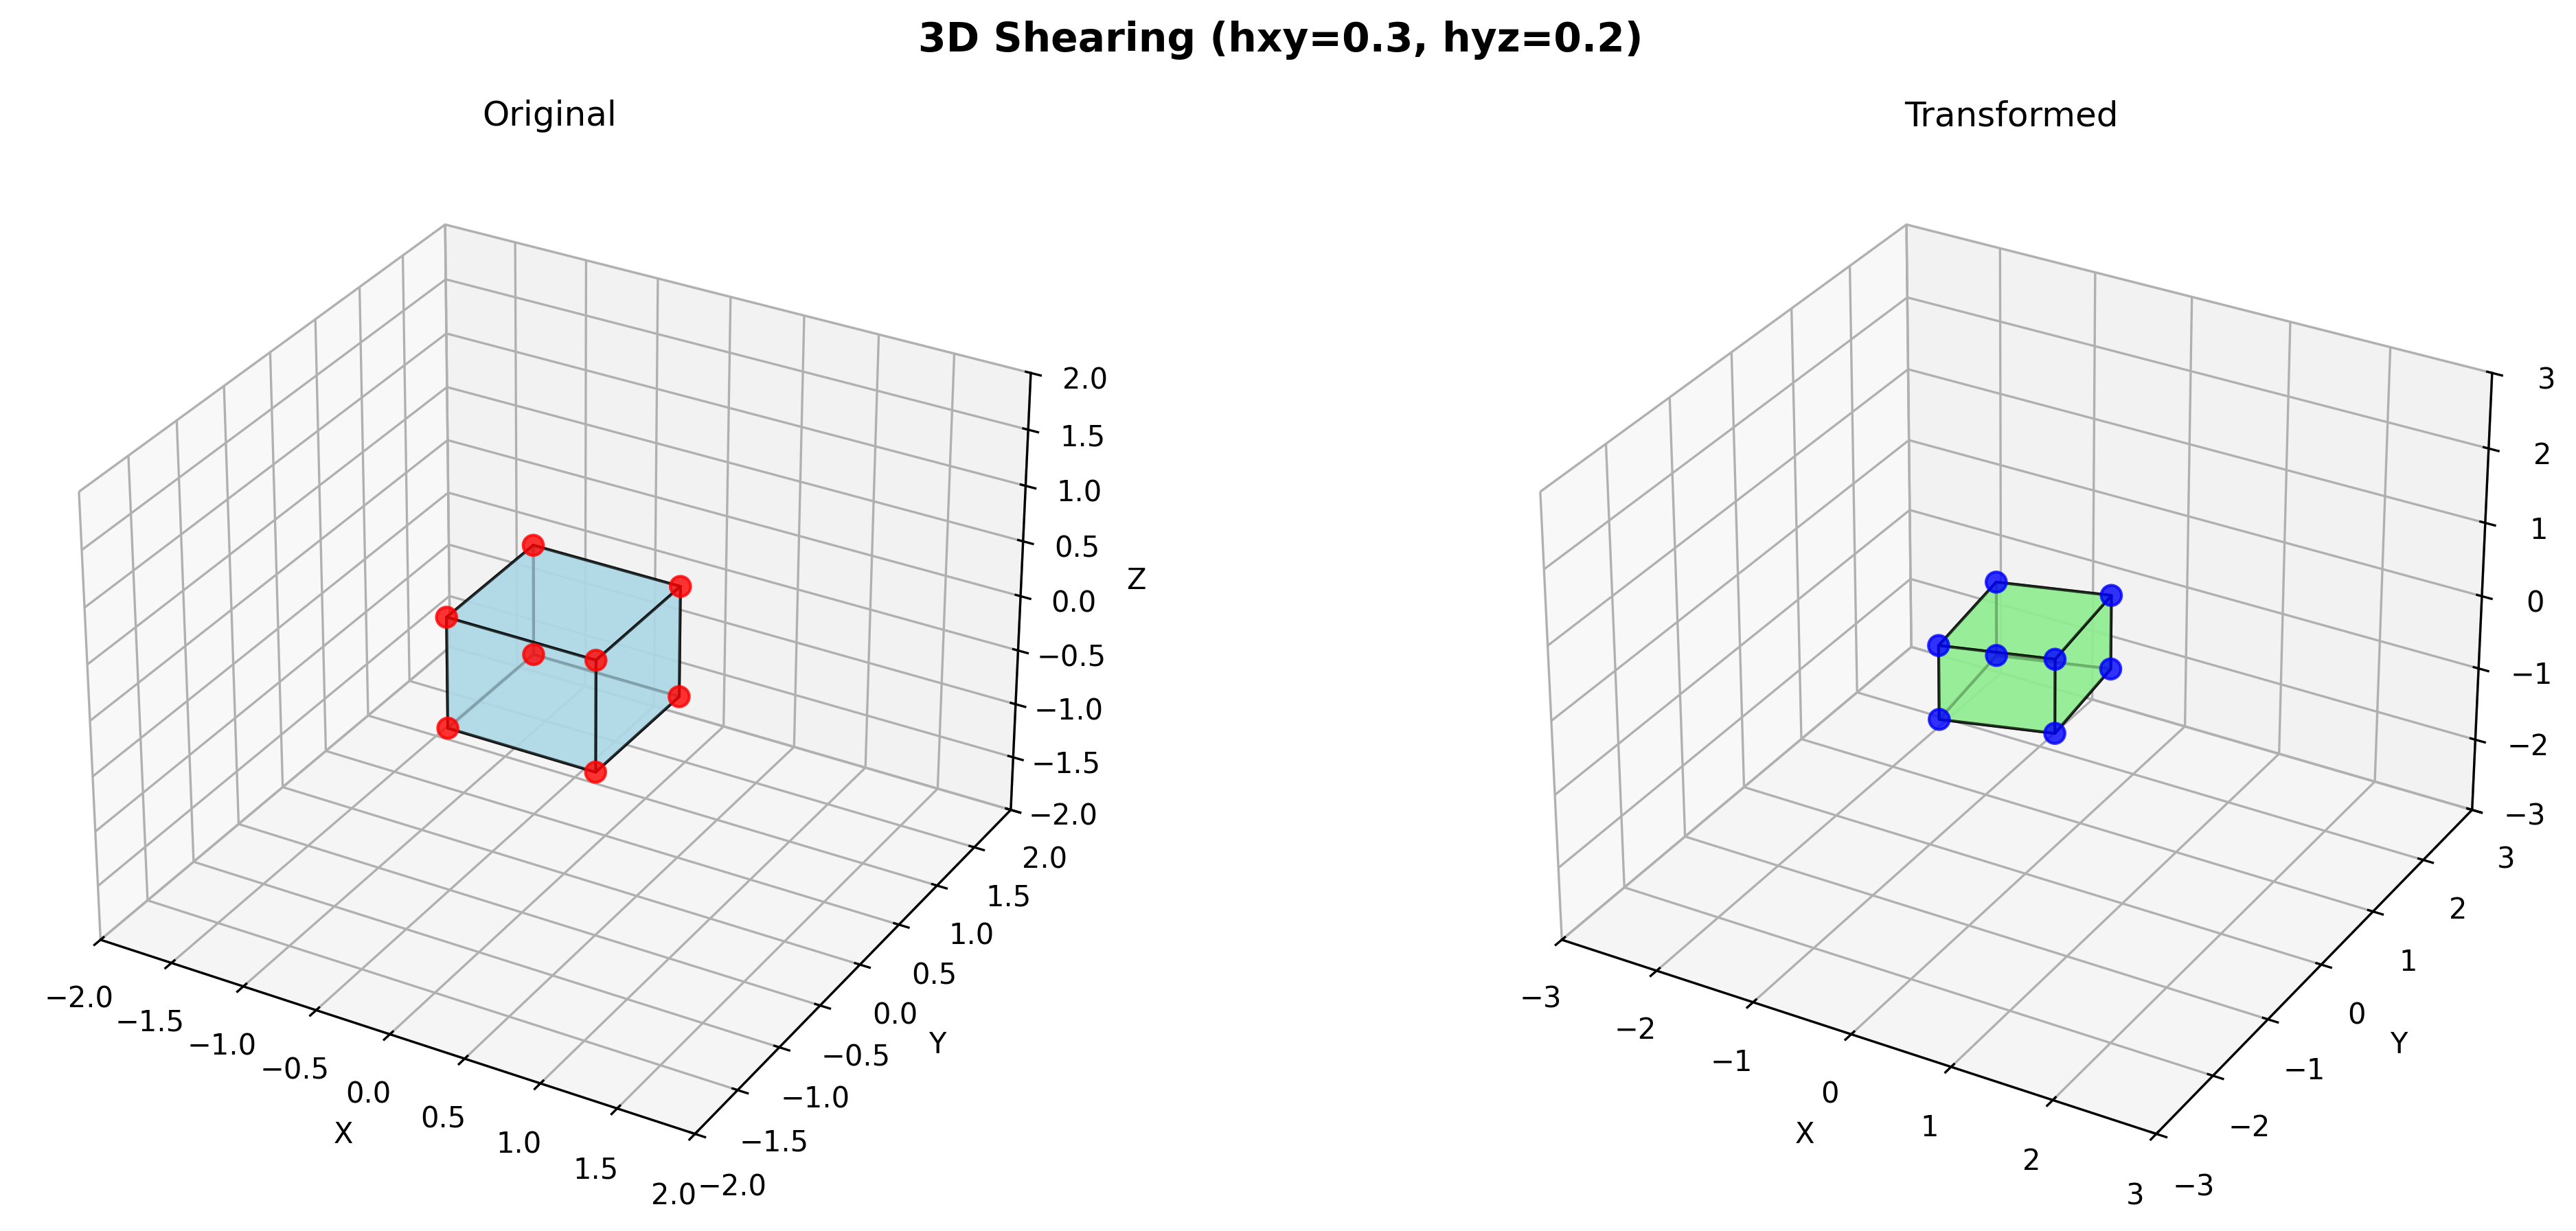
\includegraphics[width=0.8\textwidth]{fig/shearing_demo.png}
    \caption{3D Shearing demonstration showing different shearing components}
\end{figure}

\subsection{Orthographic vs Perspective Projection}
\begin{figure}[H]
    \centering
    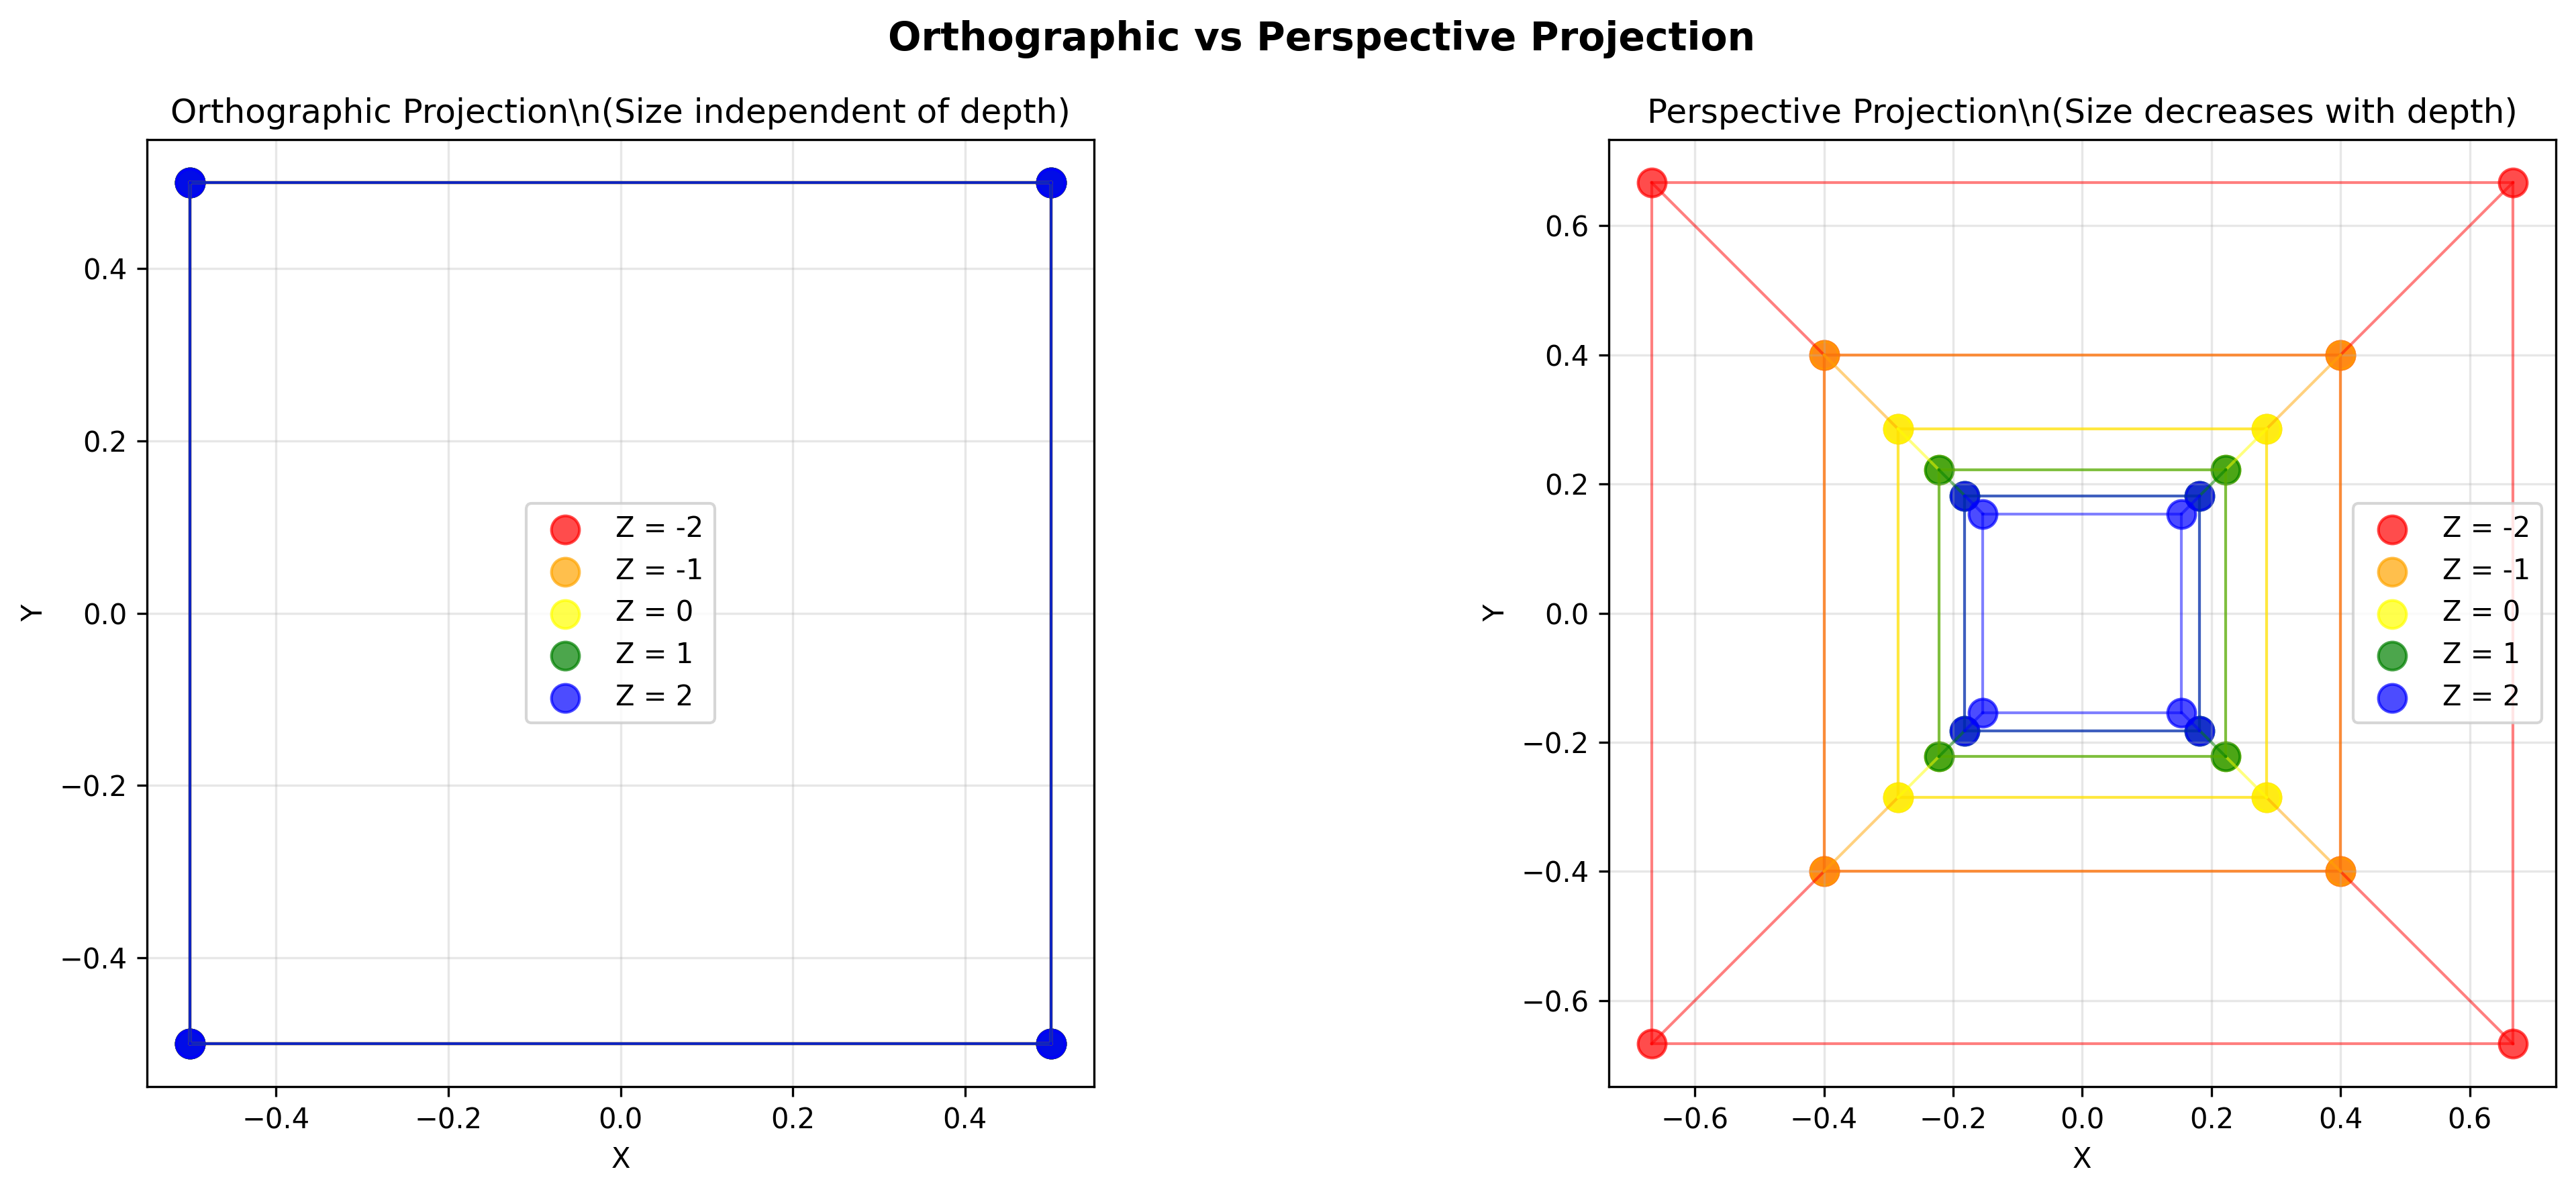
\includegraphics[width=0.8\textwidth]{fig/projection_comparison.png}
    \caption{Comparison between Orthographic and Perspective projections showing size differences}
\end{figure}

\subsection{Combined Transformations Demo}
\begin{figure}[H]
    \centering
    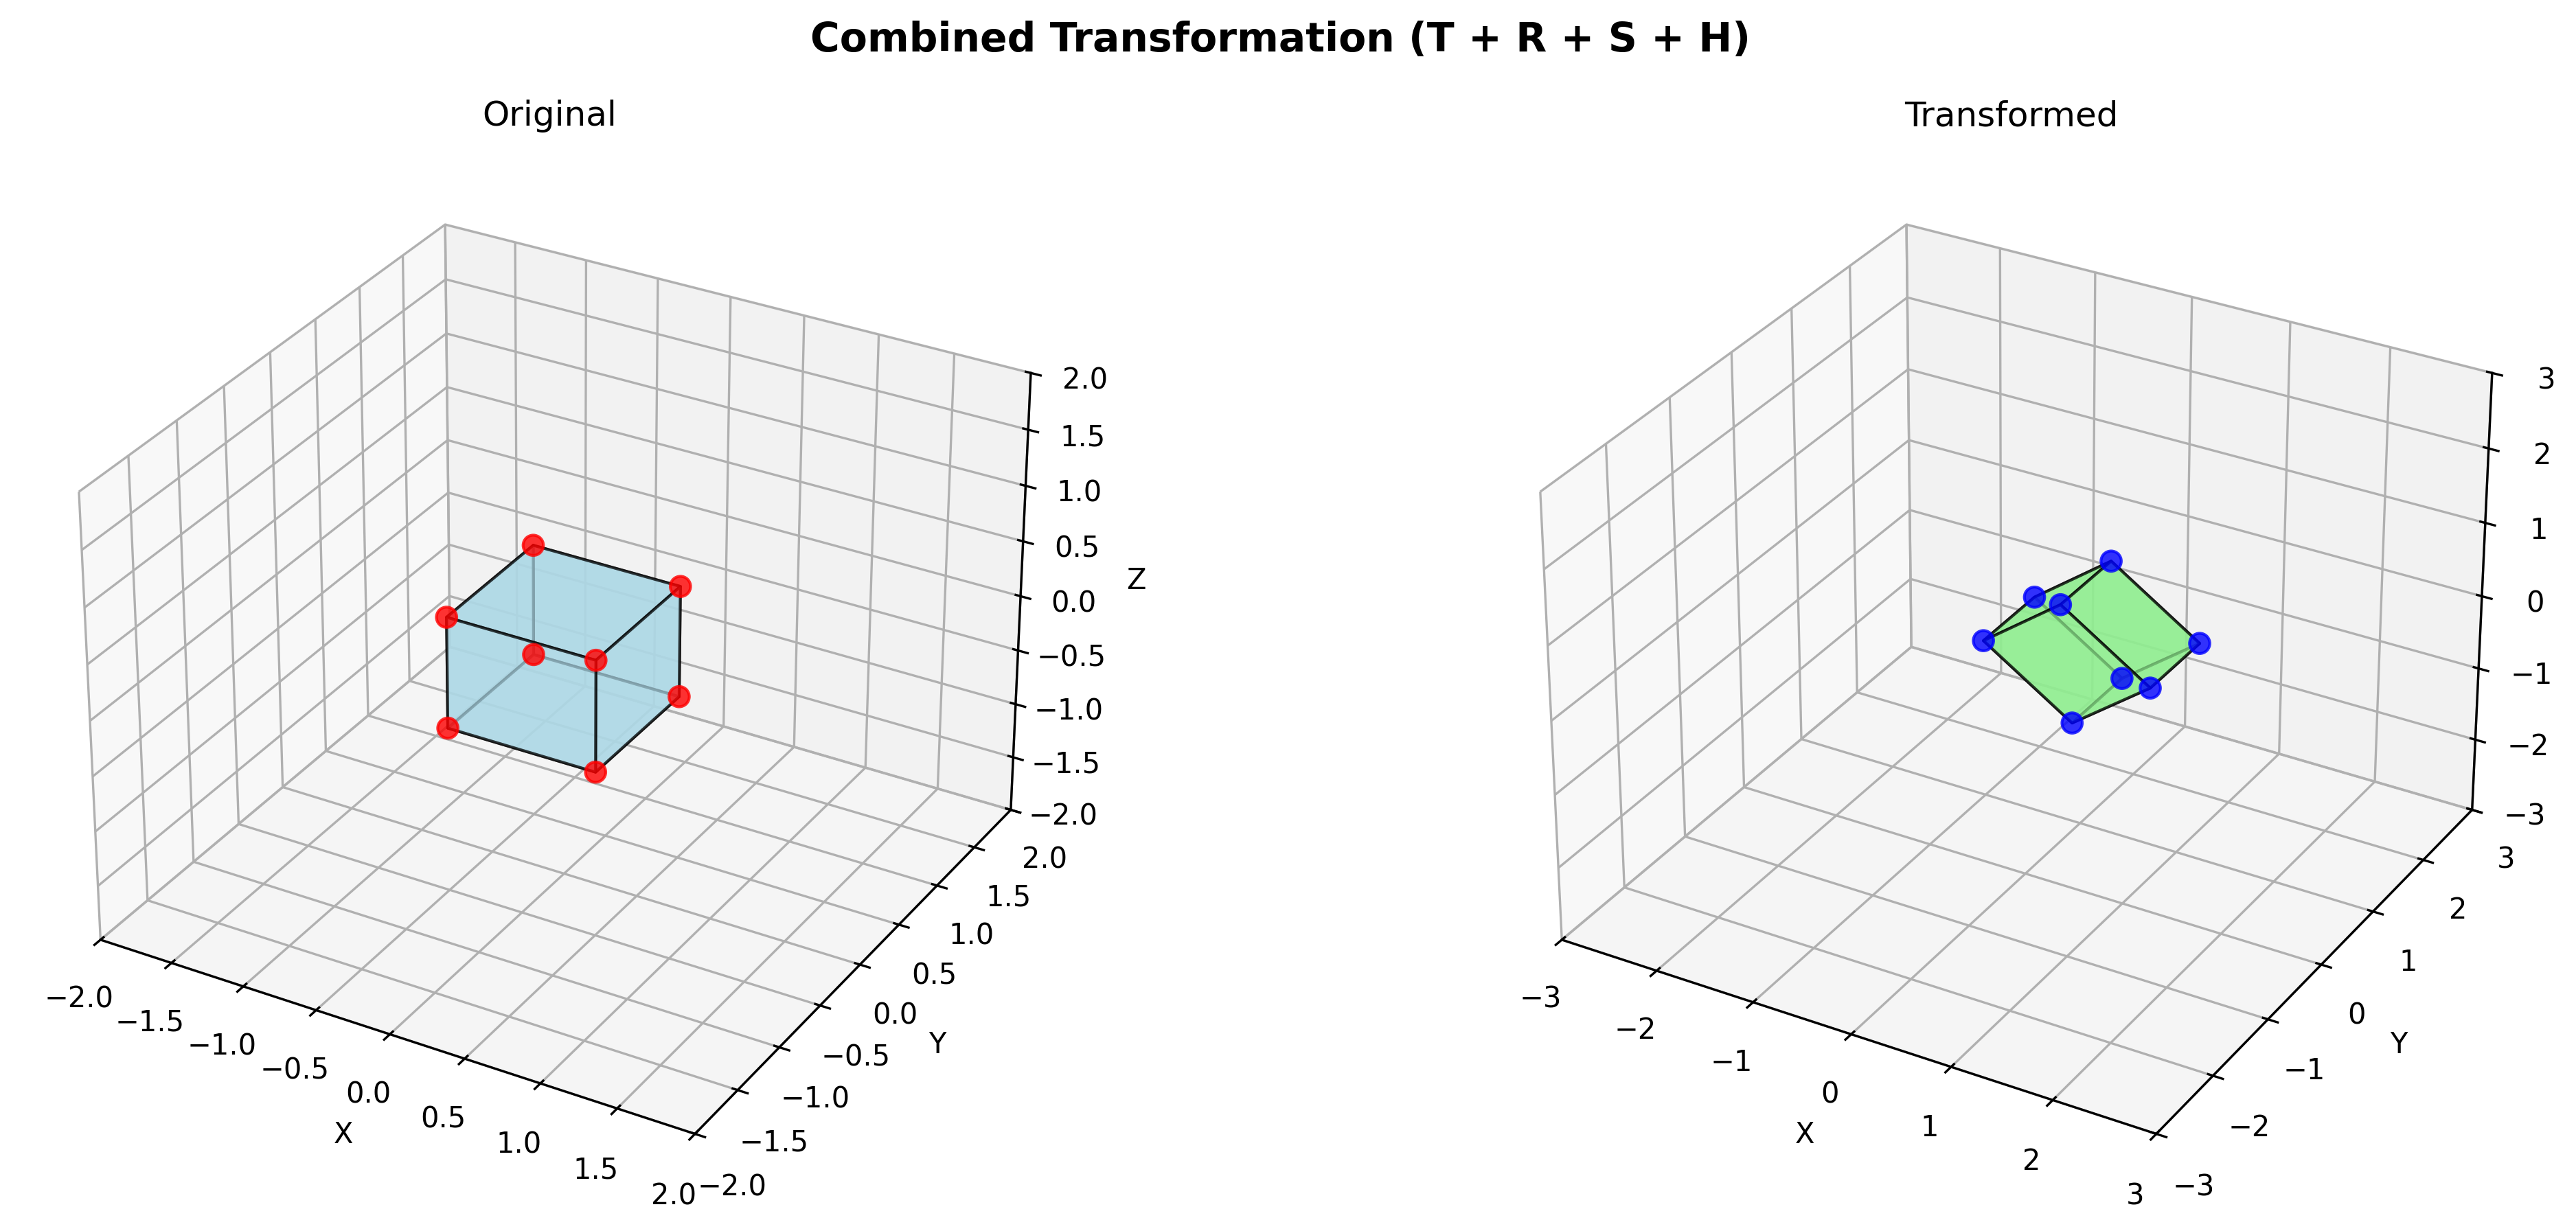
\includegraphics[width=0.8\textwidth]{fig/combined_transformation.png}
    \caption{Combined transformation demonstration showing multiple operations applied together}
\end{figure}

\section{Conclusion}

\subsection{Key Learnings}
This laboratory exercise successfully demonstrated the implementation of essential 3D transformations using OpenGL. The following key concepts were explored and implemented:

\begin{itemize}
    \item \textbf{3D Translation:} Successfully implemented translation along all three axes (X, Y, Z), allowing objects to be moved in 3D space while maintaining their orientation and shape.
    
    \item \textbf{3D Rotation:} Implemented rotation about all three principal axes. The combination of rotations about X, Y, and Z axes enables arbitrary 3D orientation of objects.
    
    \item \textbf{3D Scaling:} Demonstrated both uniform scaling (equal factors on all axes) and non-uniform scaling (different factors on different axes) to resize objects while maintaining their position.
    
    \item \textbf{3D Shearing:} Successfully implemented all six shearing components (xy, xz, yx, yz, zx, zy), providing comprehensive control over object deformation in 3D space.
    
    \item \textbf{Projection Systems:} Clearly demonstrated the fundamental difference between orthographic and perspective projections, showing how perspective projection provides depth cues while orthographic maintains parallel lines.
\end{itemize}

\subsection{Technical Achievements}

\begin{enumerate}
    \item \textbf{Matrix Transformations:} All transformations were implemented using 4×4 homogeneous transformation matrices, providing mathematical precision and enabling composition of multiple transformations.
    
    \item \textbf{Interactive Interface:} Created an intuitive keyboard-based interface allowing real-time manipulation of transformation parameters with instant visual feedback through OpenGL rendering.
    
    \item \textbf{Multiple Shape Support:} The implementation works seamlessly with various 3D primitive shapes including cubes, spheres, teapots, and tori provided by GLUT.
    
    \item \textbf{Real-time Rendering:} Achieved smooth real-time rendering with proper depth testing, lighting, and double buffering for flicker-free animation.
    
    \item \textbf{Visual Output Generation:} Implemented both OpenGL screenshot capture and matplotlib-based static visualization for comprehensive documentation and analysis.
    
    \item \textbf{Modular Design:} Organized code into separate modules for individual transformations and a comprehensive combined demo, promoting code reusability and focused learning.
\end{enumerate}

\subsection{Practical Applications}

The 3D transformations implemented in this lab form the foundation for numerous computer graphics applications:

\begin{itemize}
    \item \textbf{3D Modeling Software:} Translation, rotation, and scaling are fundamental operations in CAD and 3D modeling applications.
    
    \item \textbf{Game Development:} Real-time 3D games extensively use these transformations for character movement, object manipulation, and camera control.
    
    \item \textbf{Animation:} Keyframe animation systems rely on smooth interpolation between transformation parameters.
    
    \item \textbf{Virtual Reality:} VR applications require precise 3D transformations to create immersive experiences with accurate spatial relationships.
    
    \item \textbf{Architectural Visualization:} Different projection modes are essential for architectural rendering and technical drawings.
\end{itemize}

\subsection{Performance Considerations}

The OpenGL implementation provides excellent performance characteristics:

\begin{itemize}
    \item Hardware-accelerated matrix operations ensure smooth real-time interaction
    \item Efficient use of OpenGL state management minimizes redundant operations
    \item Proper depth buffering enables correct rendering of overlapping objects
    \item Lighting calculations add realism without significant performance impact
\end{itemize}

\subsection{Generated Visual Outputs}

This laboratory exercise successfully generated comprehensive visual documentation including:

\begin{itemize}
    \item Static transformation comparisons showing before/after states
    \item Interactive OpenGL demonstrations with real-time manipulation
    \item Projection system comparisons highlighting fundamental differences
    \item Combined transformation sequences showing complex operations
    \item Multiple 3D primitive shape demonstrations
\end{itemize}

All visual outputs are stored in the \texttt{fig/} directory and demonstrate the mathematical concepts through clear graphical representations. The visualization system provides both educational value and documentation capability for technical reports.

\subsection{File Structure and Organization}

The complete Lab 5 implementation includes:

\begin{itemize}
    \item \texttt{main.py} - Comprehensive interactive demo with all transformations
    \item \texttt{visual\_demo.py} - Static visualization generator using matplotlib
    \item \texttt{demo.py} - Quick demo runner and help system
    \item \texttt{translation.py, rotation.py, scaling.py, shearing.py} - Individual transformation demos
    \item \texttt{ortho\_projection.py} - Focused projection comparison
    \item \texttt{requirements.txt} - Python package dependencies
    \item \texttt{fig/} - Generated visual output directory with all images
\end{itemize}

\subsection{Future Enhancements}

Potential improvements and extensions to this implementation could include:

\begin{itemize}
    \item Implementation of quaternion-based rotations for smoother animation
    \item Addition of more complex transformation sequences and animation paths
    \item Integration of texture mapping and advanced lighting models
    \item Support for importing and transforming custom 3D models
    \item Implementation of advanced projection techniques like oblique projections
\end{itemize}

This laboratory exercise provided comprehensive hands-on experience with fundamental 3D computer graphics concepts, establishing a solid foundation for more advanced graphics programming topics. The combination of mathematical rigor, interactive demonstration, and comprehensive visual documentation makes this an effective learning tool for understanding 3D transformations and projection systems.

\end{document}